\chapter{Opis narzędzi i metody doboru tras}
\section{Analiza wybranego stosu technologicznego}
Aby zrealizować wymagania postawione w poprzednim rozdziale, należało wybrać odpowiedni stos technologiczny umożliwiający zbudowanie aplikacji internetowej, 
serwera oraz bazy danych obsługujące wyświetlanie, przetwarzanie oraz przechowywanie danych geograficznych.
\subsection{Technologie, narzędzia oraz biblioteki}
Wszystkie komponenty systemu zostały napisane w środowisku programistycznym \texttt{Rider} oferowanego przez firmę \emph{JetBrains}.
Systemem operacyjnym używanym podczas implementacji był \texttt{EndeavourOS} wraz z powłoką \texttt{Fish}.

Do wykonania aplikacji internetowej wykorzystano bibliotekę \texttt{React} ze względu na jej popularność, dużą społeczność oraz szeroką gamę możliwości tworzenia dynamicznych interfejsów użytkownika.
Komunikacja z serwerem odbywa się za pomocą protokołu HTTP oraz biblioteki \emph{Axios}, która ułatwia wysyłanie zapytań oraz obsługę odpowiedzi.
Wyświetlanie danych geograficznych w aplikacji internetowej realizowane jest za pomocą biblioteki \emph{Leaflet}, która umożliwia tworzenie interaktywnych map oraz dodawanie na nich znaczników.
Język \texttt{JavaScript} zastąpiono językiem \texttt{TypeScript}, który wprowadza statyczne typowanie oraz dodatkowe mechanizmy ułatwiające tworzenie i utrzymanie aplikacji.

Serwer został zaimplementowany za pomocą \texttt{ASP.NET Core}, jest to framework do tworzenia aplikacji webowych i API w języku \texttt{C\#}.
Sam model bazy danych został zdefiniowany przy użyciu \texttt{Entity Framework Core}, który umożliwia mapowanie obiektowo-relacyjne, co pozwala na łatwe odwzorowanie struktur danych w kodzie aplikacji.
Do pracy z danymi przestrzennymi wykorzystano bibliotekę \texttt{NetTopologySuite}, która integruje się z \texttt{Entity Framework Core} i umożliwia przechowywanie oraz przetwarzanie danych geograficznych w bazie danych.

Jako system relacyjnej bazy danych wykorzystano \texttt{PostgreSQL}. 
% Mam to słowo podkreślone ale w razie wątpliwości: https://dobryslownik.pl/slowo/otwarto%C5%BAr%C3%B3d%C5%82owy/225915/ 
Jest to popularny, otwartoźródłowy system, który po zainstalowaniu rozszerzeń \texttt{PostGIS} oraz \texttt{pgRouting} umożliwia przechowywanie oraz przetwarzanie danych geograficznych i tras w bazie danych.

Sam system został skonteneryzowany przy użyciu \texttt{Docker}, co umożliwia łatwe uruchamianie oraz zarządzanie wszystkimi komponentami aplikacji w izolowanych kontenerach.

Wymienione oraz pozostałe najważniejsze narzędzia wraz z ich wersjami opisano w tabelach \ref{tab:narzedzia-front}, \ref{tab:narzedzia-back} oraz \ref{tab:narzedzia-db}.
\begin{table}[htb]
\small
\centering
\caption{Wykaz narzędzi i bibliotek wykorzystanych do implementacji aplikacji internetowej}
\label{tab:narzedzia-front}
\begin{tabularx}{\linewidth}{|c|c|X|} \hline
Narzędzie & Wersja & Opis \\ \hline\hline
\texttt{TypeScript} & \texttt{7.0.2} & Język używany do implementacji aplikacji. \\ \hline
\texttt{React} & \texttt{19.3.1} & Biblioteka \texttt{JavaScript} do budowy interfejsu użytkownika w oparciu o komponenty.  \\ \hline
\texttt{Vite} & \texttt{7.1.9} & Narzędzie do uruchamiania serwera deweloperskiego oraz budowania aplikacji do wersji produkcyjnej. \\ \hline
\texttt{Node.js} & \texttt{22} & Środowisko uruchomieniowe \texttt{JavaScript} \\ \hline
\texttt{npm} & \texttt{12.2.2} & Menedżer pakietów używany do instalowania zależności i uruchamiania skryptów projektu. \\ \hline
\texttt{Material UI} & \texttt{6.4.5} & Biblioteka komponentów interfejsu dla \texttt{React}. \\ \hline
\texttt{Emotion} & \texttt{11.14.0} & Biblioteka do stylizacji komponentów wykorzystywana przez \texttt{Material UI}. \\ \hline
\texttt{Leaflet} & \texttt{1.9.4} & Biblioteka map oraz jej integracja z komponentami \texttt{React}. \\ \hline
\texttt{Axios} & \texttt{1.7.2} & Biblioteka do wykonywania żądań HTTP do API. \\ \hline
\end{tabularx}
\end{table}

\begin{table}[htb]
\small
\centering
\caption{Wykaz narzędzi i bibliotek wykorzystanych do implementacji serwera}
\label{tab:narzedzia-back}
\begin{tabularx}{\linewidth}{|c|c|X|} \hline
Narzędzie & Wersja & Opis \\ \hline\hline
\texttt{C\#} & \texttt{14} & Język programowania używany do implementacji serwera.  \\ \hline
\texttt{ASP.NET Core} & \texttt{10.0} & Framework do API  \\ \hline
\texttt{Entity Framework Core} & \texttt{10.0.14} & ORM do mapowania obiektów na dane oraz obsługi dostępu do bazy danych.  \\ \hline
\texttt{Scalar.AspNetCore} & \texttt{2.18.7} & Interfejs dokumentacji i eksploracji API, zintegrowany z ASP.NET Core.  \\ \hline
\texttt{NetTopologySuite} & \texttt{10.0.3} & Obsługa typów i operacji danych przestrzennych używana z PostgreSQL.  \\ \hline
\texttt{DispatchR.Mediator} & \texttt{2.3.1} & Biblioteka implementująca wzorzec mediator do przekazywania i obsługi żądań w aplikacji.  \\ \hline
\texttt{Bogus} & \texttt{35.6.5} & Biblioteka do generowania przykładowych i testowych danych.  \\ \hline
\texttt{IdentityModel.Tokens} & \texttt{8.23.0} & Biblioteka do tworzenia i weryfikacji tokenów JWT.  \\ \hline
\texttt{CsvHelper} & \texttt{33.1.0} & Biblioteka do odczytu i zapisu danych w formacie CSV.  \\ \hline
\end{tabularx}
\end{table}

\begin{table}[htb]
\small
\centering
\caption{Wykaz systemów i narzędzi wykorzystanych do implementacji i obsługi bazy danych}
\label{tab:narzedzia-db}
\begin{tabularx}{\linewidth}{|c|c|X|} \hline
Narzędzie & Wersja & Opis \\ \hline\hline
\texttt{PostgreSQL} & \texttt{18.6} & Relacyjny system zarządzania bazą danych.  \\ \hline
\texttt{PostGIS} & \texttt{3.6} & Rozszerzenie PostgreSQL umożliwiające przechowywanie i przetwarzanie danych przestrzennych.  \\ \hline
\texttt{pgRouting} & \texttt{4.0.1} & Rozszerzenie PostgreSQL/PostGIS udostępniające funkcje i algorytmy wykorzystywane do doboru tras.  \\ \hline
\texttt{osm2po} & \texttt{5.5.14} & Narzędzie przetwarzające dane OpenStreetMap i przygotowujące graf drogowy do wykorzystania w obliczeniach tras.  \\ \hline
\end{tabularx}
\end{table}

\subsection{Wzorce projektowe}
Skalowalność i łatwość konserwacji oprogramowania to najważniejsze atrybuty nowoczesnych systemów. 
W celu ich osiągnięcia zastosowano wzorce projektowe, które pozwoliły na uzyskanie wyżej wymienionych cech.

\textbf{CQRS (ang.~\emph{Command Query Responsibility Segregation})} to wzorzec projektowy, który rozdziela operacje modyfikujące stan systemu (komendy) od operacji odczytujących dane (zapytania) \cite{MS_CQRS}.
W zaimplementowaniu tego wzorca użyto biblioteki \texttt{DispatchR}, która udostępnia mechanizm oparty o wzorzec mediatora pozwalający na obsługę komend i zapytań w sposób scentralizowany.
Pozwala to na lepszą skalowalność i czytelność kodu. Zastosowanie tego wzorca w projekcie pokazano na przykładzie folderu \texttt{Routes} w module \texttt{Eider-Rider.Core}.
\begin{lstlisting}[label=list:cqrsExample,caption=Przykład zastosowania wzorca CQRS w module Routes,style=folderview]
Eider-Rider.Core
|-- Routes
|   |-- Abstractions
|   |   \-- IRouteMatchingService.cs
|   |-- Commands
|   |   |-- CreateRouteCommand.cs
|   |   \-- DeleteRouteByIdCommand.cs
|   |-- Queries
|   |   |-- GetAllRoutesByUserIdQuery.cs
|   |   \-- GetMatchedRouteQuery.cs
|   |-- Results
|   |   \-- RouteDto.cs
|   \-- Services
|       |-- RouteLengthCalculator.cs
|       \-- RouteMatchingService.cs
\-- ServiceExtensions.cs
\end{lstlisting}
\subsection{Wzorzec rozszerzenia serwisów}
W każdym module systemu znajduje się plik \texttt{ServiceExtensions.cs}, który zawiera metody rozszerzające dla serwisów zdefiniowanych w danym module. 
Dzięki temu plik \texttt{Program.cs} w module \texttt{Eider-Rider.Api} nie musi wywoływać konfiguracji każdego serwisu, jedynie wywołuje metody rozszerzające zdefiniowane w poszczególnych modułach.
Zmniejsza to jego objętość i poprawia czytelność kodu.
Sam wzorzec polega na stworzeniu statycznej metody zwracającej \texttt{IServiceCollection}, która rejestruje i konfiguruje serwisy w kontenerze zależności \cite{SERVICE_EXTENSIONS}.
Następnie wystarczy wywołać tę metodę w pliku \texttt{Program.cs}.
\begin{lstlisting}[label=list:serviceExtensionsExample,caption=Przykład zastosowania wzorca rozszerzenia serwisów,style=sharpcstyle]
public static class ServiceExtensions
{
    public static IServiceCollection AddAuthServices(this IServiceCollection services, IConfiguration configuration)
    {
        services.AddOptionsWithRequiredFieldsValidation<JwtSettings>(configuration);
        
        services.AddScoped<IRefreshTokenService, RefreshTokenService>();
        services.AddScoped<ITokenService, TokenService>();
        
        return services;
    }
}
\end{lstlisting}
\subsection{Wzorzec opcji}
Zamiast bezpośredniego wpisywania ustawień JWT w kodzie, wykorzystuje się wzorzec opcji, który pozwala na mapowanie ustawień z pliku konfiguracyjnego do obiektu w kodzie.
Uwierzytelnianie i autoryzacja w systemie opiera się na \texttt{JWT}, którego ustawienia są przechowywane w pliku \texttt{appsettings.json}.
W pliku \texttt{Program.cs} w module \texttt{Eider-Rider.Api} można następnie wstrzyknąć ustawienia JWT do serwisów, które ich potrzebują.
Klasa \texttt{JwtSettings} definiuje strukturę ustawień JWT, które są następnie wykorzystywane przez klasę \texttt{TokenService}, pełni on rolę serwisu
odpowiedzialnego za generowanie tokenów JWT.
\begin{lstlisting}[label=list:optionsExample,caption=Przykład zastosowania wzorca opcji w kontekście ustawień JWT,style=sharpcstyle]
public class JwtSettings : IEiderRiderOptions
{
    public static string SectionName => "JwtSettings";
    
    [Required]
    public required string Key { get; init; }
    [...]
}
\end{lstlisting}
\subsection{Mediator}
W pewnym momencie rozwoju systemu liczba zależności między modułami rośnie do momentu, w którym przedstawienie jego struktury na diagramie i utrzymywanie go przestaje mieć sens.
Mediator to behawioralny wzorzec projektowy pozwalający zredukować sprzężenie pomiędzy komponentami programu poprzez zmuszenie ich do komunikacji za pośrednictwem obiektu zwanego mediatorem.
Jak wspomniano przy opisie wzorca CQRS, mediator został wykorzystany do scentralizowanej obsługi komend i zapytań.
Mediator ułatwia modyfikację, rozszerzanie i ponowne wykorzystanie komponentów.
\begin{figure}[h]
	\centering
	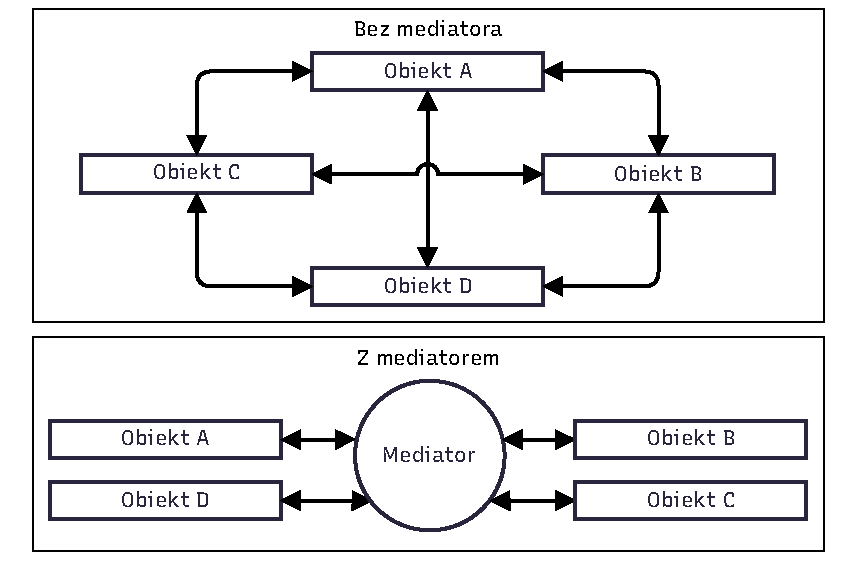
\includegraphics[width=0.9\linewidth]{rys03/Mediator_comparison.drawio_cropped.pdf}
	\caption{Przykład zastosowania wzorca mediatora}
	\label{fig:mediator_comparison}
\end{figure}

Komenda lub zapytanie wykorzystywane przez mediatora musi implementować interfejs \texttt{IRequest}, który określa typ odpowiedzi zwracanej przez mediatora.
Interfejs \texttt{IRequestHandler} definiuje metodę \texttt{Handle}, która jest wywoływana przez mediatora w celu obsługi danej komendy lub zapytania.
Klasa implementująca ten interfejs musi określić typ komendy lub zapytania, które obsługuje, oraz typ odpowiedzi, którą zwraca metoda \texttt{Handle}.
Na tej podstawie mediator znajduje odpowiedni handler dla danej komendy lub zapytania i wywołuje metodę \texttt{Handle}.
\begin{lstlisting}[label=list:mediatorExample,caption=Przykład komendy i handlera we wzorcu mediatora,style=sharpcstyle]
public record CreateCarCommand : IRequest<CreateCarCommand, Task<Guid>>
{[...]}

internal sealed class CreateCarCommandHandler : IRequestHandler<CreateCarCommand, Task<Guid>>
{
    private readonly EiderRiderDbContext _dbContext;

    public CreateCarCommandHandler(EiderRiderDbContext dbContext)
    {
        _dbContext = dbContext;
    }

    public async Task<Guid> Handle(CreateCarCommand request, CancellationToken cancellationToken)
    {
        var newCar = new CarEntity
        {[...]};
        
        _dbContext.Add(newCar);
        await  _dbContext.SaveChangesAsync(cancellationToken);
        
        return newCar.Id;
    }
}
\end{lstlisting}

Na przykładzie przedstawionym na rysunku \ref{fig:mediator_sequence} pokazano jak przebiega interakcja pomiędzy kontrolerem, mediatorem oraz odpowiednim handlerem obsługującym komendę oraz bazą danych.
Klient wysyła żądanie w postaci \texttt{CreateCarRequest} do kontrolera \texttt{CarController}, który przekłada je na komendę \texttt{CreateCarCommand} i przekazuje do mediatora za pomocą jego metody \texttt{Send}.
Mediator następnie przekazuje komendę do odpowiedniego handlera posiadającego metodę \texttt{Handle}, która realizuje logikę biznesową związaną z tworzeniem samochodu.
\begin{figure}[h]
	\centering
	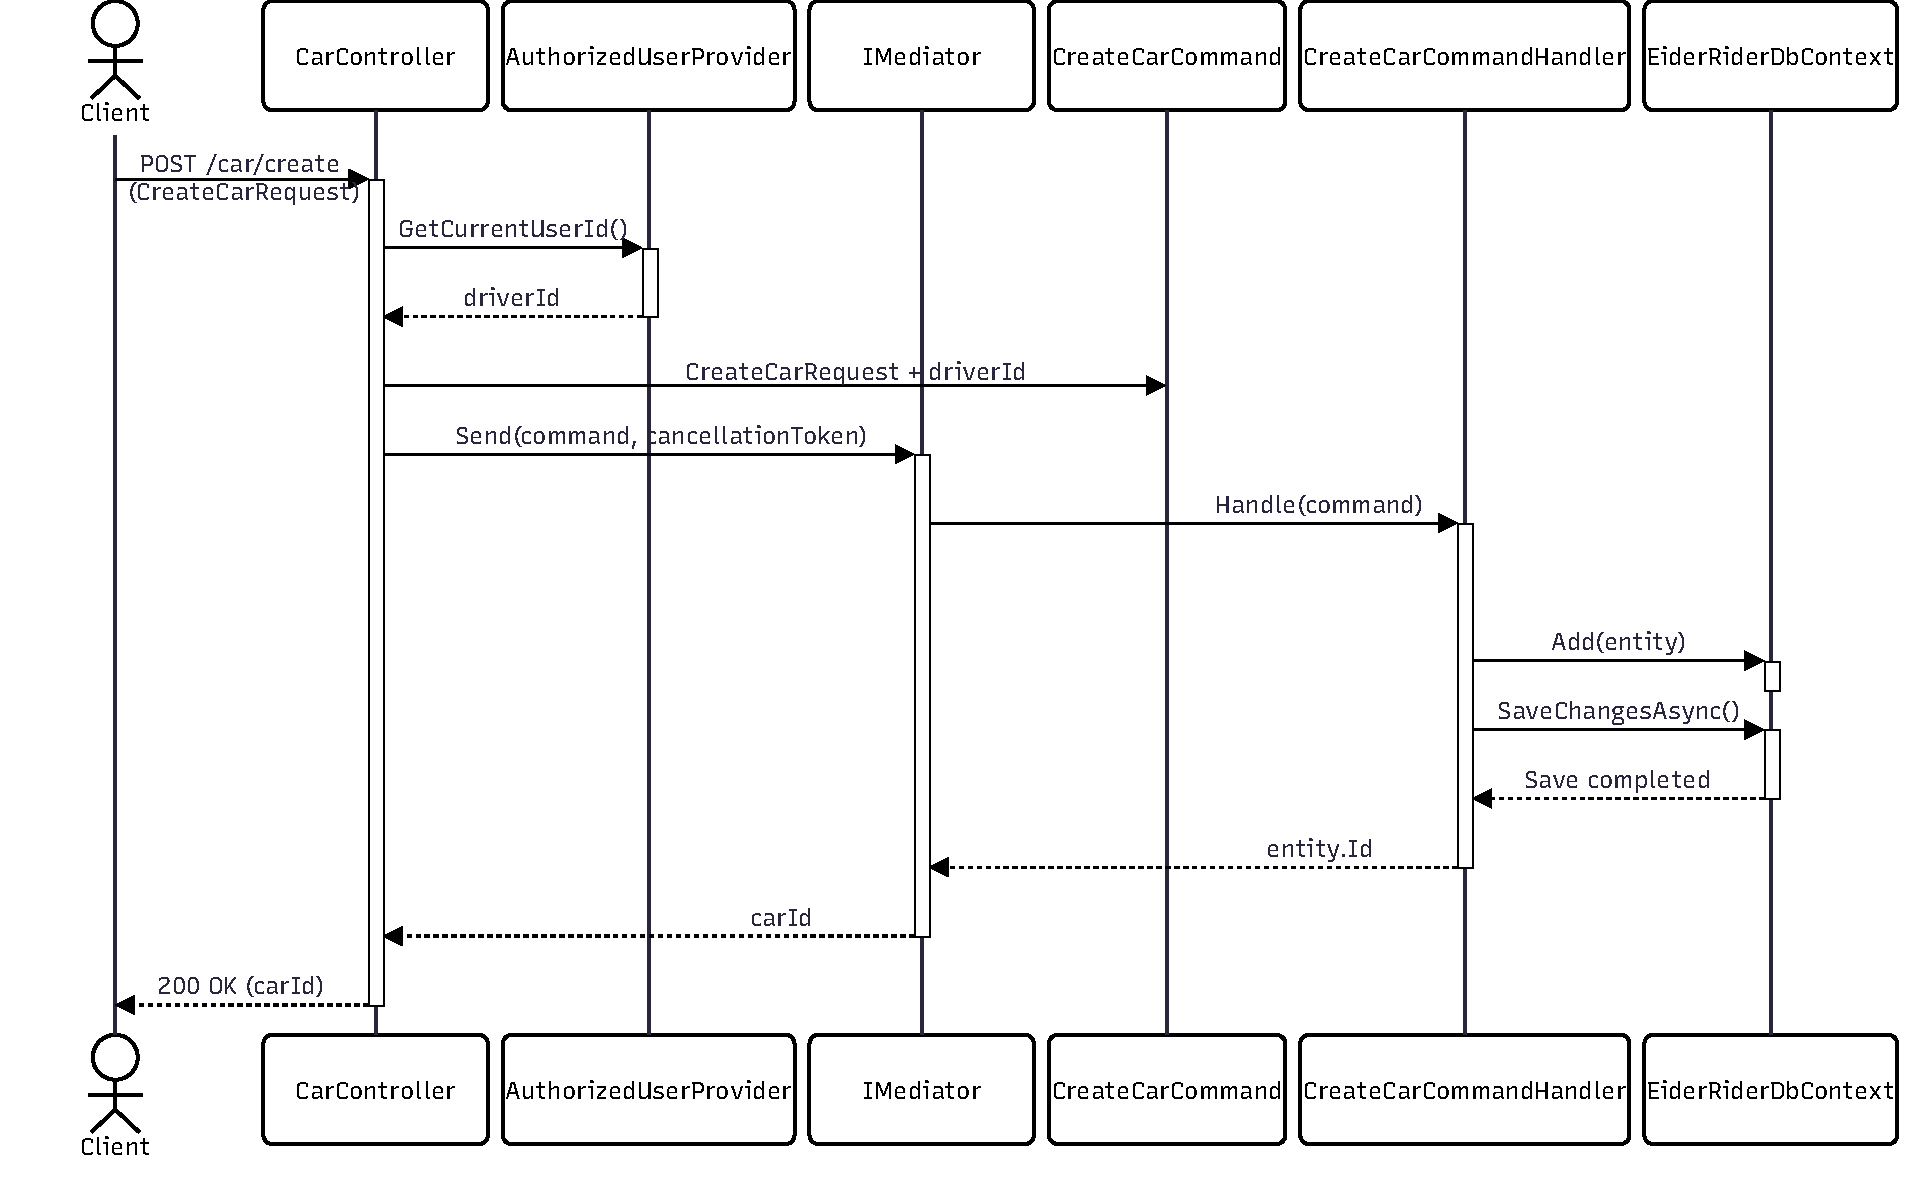
\includegraphics[width=1\linewidth]{rys03/Mediator_sequence.drawio.pdf}
	\caption{Diagram interakcji mediatora na przykładzie funkcji tworzenia samochodu}
	\label{fig:mediator_sequence}
\end{figure}
\section{Opis algorytmu doboru pasażerów do kierowców}

\subsection{Przebieg algorytmu}
\begin{enumerate}
    \item Odfiltrowanie dostępnych tras na podstawie następujących kryteriów:
    \begin{itemize}
        \item Czas odjazdu nie minął.
        \item Czas przyjazdu kierowcy do celu jest wcześniejszy niż docelowy czas przyjazdu pasażera.
        \item Miejsce początkowe i końcowe kierowcy jest w promieniu wyszukiwania wyznaczonym przez pasażera.
        \item W samochodzie kierowcy znajdują się miejsca wolne (określone na podstawie zaakceptowanych rezerwacji na dany przejazd).
    \end{itemize}
    \item Wstępne posortowanie odfiltrowanych tras na podstawie sumy odległości w linii prostej pomiędzy punktami początkowymi i końcowymi kierowcy oraz pasażera.
    \item Przygotowanie reprezentacji grafu sieci drogowej.
    \item Dopasowanie podanych przez użytkowników punktów do najbliższych wierzchołków w grafie.
    \item Wyznaczenie rzeczywistej drogi dojazdu w sieci drogowej przy użyciu algorytmu Dijkstry.
    \begin{itemize}
        \item Obliczenie odległości od punktu początkowego pasażera do punktów początkowych tras kierowców
        \item Obliczenie odległości od punktów końcowych tras kierowców do punktu docelowego pasażera
    \end{itemize}
    \item Zsumowanie obu kosztów dla każdej z rozpatrywanych tras, posortowanie wyników rosnąco według łącznej odległości oraz wybór najlepszej trasy.
    \item Pobranie pełnych danych wybranej trasy z bazy danych i zwrócenie jej w postaci obiektu \texttt{RouteDto} lub \texttt{null} w przypadku braku odpowiedniej trasy.
\end{enumerate}
\subsection{Implementacja algorytmu}